\documentclass[italian,a4paper]{article}
\usepackage[tight,nice]{units}
\usepackage{babel,amsmath,amssymb,amsthm,graphicx,url}
\usepackage[text={5.5in,9in},centering]{geometry}
\usepackage[utf8x]{inputenc}
\usepackage[T1]{fontenc}
\usepackage{ae,aecompl}
\usepackage[footnotesize,bf]{caption}
\usepackage[usenames]{color}
\usepackage{textcomp}
\usepackage{gensymb}
%\include{pstricks}
\frenchspacing
\pagestyle{plain}
%------------- eliminare prime e ultime linee isolate
\clubpenalty=9999%
\widowpenalty=9999
%--- definizione numerazioni
\renewcommand{\theequation}{\thesection.\arabic{equation}}
\renewcommand{\thefigure}{\arabic{figure}}
\renewcommand{\thetable}{\arabic{table}}
\addto\captionsitalian{%
  \renewcommand{\figurename}%
{Grafico}%
}
%
%------------- ridefinizione simbolo per elenchi puntati: en dash
%\renewcommand{\labelitemi}{\textbf{--}}
\renewcommand{\labelenumi}{\textbf{\arabic{enumi}.}}
\setlength{\abovecaptionskip}{\baselineskip}   % 0.5cm as an example
\setlength{\floatsep}{2\baselineskip}
\setlength{\belowcaptionskip}{\baselineskip}   % 0.5cm as an example
%--------- comandi insiemi numeri complessi, naturali, reali e altre abbreviazioni
\renewcommand{\leq}{\leqslant}
%--------- porzione dedicata ai float in una pagina:
\renewcommand{\textfraction}{0.05}
\renewcommand{\topfraction}{0.95}
\renewcommand{\bottomfraction}{0.95}
\renewcommand{\floatpagefraction}{0.35}
\setcounter{totalnumber}{5}
%---------
%
\newcommand{\Z}{\mathbb{Z}}

%---------
\begin{document}
\title{Relazione di laboratorio: Analisi di figure di diffrazione e interferenza}
\author{\normalsize Ilaria Brivio (582116)\\
\normalsize \url{brivio.ilaria@tiscali.it}
\and 
\normalsize Matteo Abis (584206)\\ 
\normalsize \url{webmaster@latinblog.org}}
\date{\today}
\maketitle
%------------------
\section{Obiettivo dell'esperienza}
Obiettivo dell'esperienza è l'analisi delle figure di interferenza prodotte da un fascio luminoso che attraversa un sistema di poche fenditure per dare una stima dell'ampiezza della singola fenditura e della distanza tra due di esse.
% Si vuole inoltre verificare la propozionalità dell'intensità luminosa del segnale raccolto dal quadrato del numero di fenditure.

\section{Descrizione dell'apparato strumentale}
L'apparato è costituito da diversi elementi posizionati su un banco ottico: una sorgente, un supporto per il sistema di fenditure e un braccio meccanico sulla cui estremità libera è montato un rivelatore.

La sorgente è un laser che emette luce monocromatica di lunghezza d'onda $\lambda=\unit[670]{nm}$ con una potenza di circa \unit[0.3]{mW}. Le fenditure sono impresse su una lamina di acetato a gruppi di una, due, tre e quattro. Tale lamina è montata su un telaio che può essere traslato ortogonalmente al banco ottico con una vite micrometrica, in modo da poter illuminare il numero di fenditure scelto.

Il braccio meccanico è fissato ad un'estremità al banco ottico e ruota attorno a questa grazie a una vite senza fine di passo $p=\unit[0.5]{mm}$ posta a distanza $\ell=\unit[65.5 \pm 0.5]{mm}$ dal centro di rotazione. La vite è azionata da un motore che compie 400 passi per ogni giro di vite (1 passo =\unit[1.25]{\micro m}). All'altra estremità del braccio è fissato un fotodiodo che rileva l'intensità del segnale luminoso in scala logaritmica.

Motore e rivelatore sono gestiti dallo sperimentatore attraverso un programma che permette di controllare la posizione e i movimenti del braccio e che registra i valori dell'intensità luminosa in corrispondenza della posizione del motore.
\subsection*{Osservazioni sulle misure di intensità luminosa}
Dall'ingrandimento dei grafici realizzati con i dati di intensità luminosa (si veda ad esempio il grafico~\ref{dentini}) si osserva che le misure effettuate dal fotodiodo hanno un andamento molto regolare, con fluttuazioni di ampiezza pressoché costante (circa cinque unità) con un periodo di quattro \emph{step}, legate verosimilmente alla struttura intrinseca dello strumento, e senza rilevanza per la fisica di questo esperimento

Tali fluttuazioni potrebbero costituire una fonte di errore sulla determinazione delle posizioni e dei valori di intensità dei minimi di interferenza. Tuttavia l'analisi fornita dalla libreria TSpectrum di ROOT esegue un buon lavoro nell'interpretazione del rumore elettronico, essendo appositamente programmata, quindi ci aspettiamo che tale errore sia del tutto irrilevante rispetto a quello sulle altre misure.

Le figure di interferenza, inoltre, sembrano presentare una certa asimmetria. Abbiamo eseguito una misura del fondo luminoso, con il laser spento, per verificare che non fosse dovuta all'illuminazione della stanza. Come si può vedere dai grafici~\ref{fondo_scan} e~\ref{fondo}, il fondo luminoso sembra perfettamente costante lungo l'escursione del braccio considerata, da -2300 a +2300 step intorno al massimo centrale. Si nota anche qui la stessa struttura periodica nella rilevazione delle intensità, e il grafico~\ref{fondo} ci permetterebbe di dare una stima nell'ampiezza delle oscillazioni, che sono una verosimile stima dell'errore sulla misura delle intensità, con un RMS di 2.

\section{Descrizione della metodologia di misura}
\`{E} stata dapprima illuminata con il laser la fenditura singola e sono state effettuate le misure facendo ruotare il braccio meccanico attorno alla posizione parallela al banco ottico, partendo da una posizione corrispondente a -2300 passi del motore fino a +2300. \`{E} stato acquisito un valore dell'intensità luminosa per ogni passo del motore.

Lo stesso procedimento è stato ripetuto illuminando successivamente due, tre o quattro fenditure.
\section{Risultati sperimentali ed elaborazione dati}
\subsection*{Diffrazione da singola fenditura}
\`{E} stata misurata l'intensità luminosa raccogliendo un valore per ogni passo del motore dalla posizione di -2300 passi a quella di +2300. I valori raccolti sono stati riportati in grafico~\ref{1slitint}.

Dopo aver estrapolato le ascisse dei minimi con l'apposita libreria TSpectrum di ROOT, sono stati calcolati i corrispondenti angoli di deflessione $\theta$, secondo la relazione:
\begin{equation*}
\theta = x \:\dfrac{\unit[1.25]{\micro m}}{\ell}
\end{equation*}
dove $x$ è il numero di step del motore, \unit[1.25]{\micro m} è lo spostamento della vite per il singolo step e $\ell=\unit[65.5 \pm 0.5]{mm}$ la distanza della vite dal centro di rotazione.

Dall'analisi teorica del fenomeno della diffrazione ci si aspetta che l'intensità vari con $\theta$ secondo la relazione
\begin{equation*}
I(\theta)=I_0\left[\dfrac{\sin{\left(\pi\frac{a}{\lambda}\sin\theta\right)}}{\pi\frac{a}{\lambda}\sin\theta}\right]^2
\end{equation*}
e dunque che l'$n$-esimo minimo di intensità corrisponda a
\begin{equation*}
\sin{\theta} = n\dfrac{\lambda}{a},\quad n \in \Z
\end{equation*}
\`{E} stato quindi realizzato un grafico con i numeri d'ordine dei minimi ($n$) in ascissa e i valori di $\sin\theta$ in ordinata (Grafico~\ref{1slitsin}) e sono stati interpolati linearmente, con due rette distinte, i dati relativi ai minimi alla sinistra e alla destra del massimo centrale.

Si è ricavata poi la misura dell'ampiezza della fenditura come $a = \lambda/m$, dove $m$ è il coefficiente angolare della retta interpolante. Gli errori sui parametri del fit sono stati calcolati a posteriori con un test del chi quadro, cercando di ottenere un valore per $\chi^2$ il più possibile vicino a uno. Da questi sono stati poi ottenuti quelli su $a$ da $\sigma_a/a=\sigma_m/m$, avendo assunto come nullo l'errore su $\lambda$.

L'operazione è stata ripetuta per ciascuna delle due interpolazioni, trovando così due stime di $a$. Come valore finale si è infine assunta la media pesata:
\begin{equation*}
a=\unit[80.6 \pm 0.2]{\micro m}
\end{equation*}

\subsection*{Interferenza da più fenditure}
Le misure di intensità raccolte per le figure di interferenza da due, tre e quattro fenditure sono state riportate nei tre grafici in appendice (Grafici~\ref{2slitsint},~\ref{3slitsint},~\ref{4slitsint}).

Dato che la lunghezza del braccio meccanico è molto maggiore delle dimensioni del sistema di fenditure, possiamo con ottima approssimazione assumere che siano soddsifatte le condizioni di Fraunhofer di sorgenti coerenti e lontane. A meno di un fattore di forma legato agli effetti di diffrazione, l'intensità segue perciò l'andamento dato da:
\begin{equation*} 
I(\phi)=I_0\left[\dfrac{\sin\left(N\phi/2\right)}{\sin\left(\phi2\right)}\right]^2
\end{equation*}
dove $N$ è il numero di fenditure del sistema e $\phi$ è la differenza di fase tra due sorgenti. Essendo queste ultime coerenti e poste a distanza $d$ l'una dall'altra, si ha in particolare
\begin{equation*}
\phi= 2\pi \dfrac{d}{\lambda}\sin\theta 
\end{equation*}
Dunque per
\begin{equation*}
\dfrac{\phi}{2}=k\pi\qquad\Rightarrow\qquad \sin\theta= k \dfrac{\lambda}{d},\quad k \in \Z
\end{equation*}
si avranno i massimi principali, mentre per
\begin{equation*}
\dfrac{\phi}{2}=\dfrac{n\pi}{N}\qquad\Rightarrow\qquad\sin\theta=n\dfrac{\lambda}{Nd},\quad n \in \Z
\end{equation*}
si avranno dei minimi. In particolare tra due massimi principali, che cadono ogniqualvolta $n/N$ è un intero, ci saranno $N-1$ minimi.

Sono state dunque estrapolate le ascisse dei minimi di intensità e ne sono stati calcolati gli angoli di deflessione $\theta$, analogamente a quanto fatto per la diffrazione da singola fenditura.
I valori di $\sin\theta$ sono stati posti in grafico in relazione al numero d'ordine dei minimi (Grafici~\ref{2slitssin},~\ref{3slitssin},~\ref{4slitssin}).
Avendo osservato che lontano dal centro alcuni minimi non sono stati rilevati correttamente, ad esempio perché interpretati come flessi, sono stati scartati tutti gli ordini dall'irregolarità in poi.

I punti relativi ai minimi alla sinistra e alla destra del massimo centrale sono stati interpolati linearmente con due rette distinte e da ciascuno dei due coefficienti angolari si è ricavata una stima della distanza $d=\lambda/(mN)$ tra le fenditure.
Come valore finale per $d$ si è assunta la media pesata, mentre l'errore è stato ottenuto con lo stesso metodo impiegato in precedenza per la diffrazione.

L'operazione è stata ripetuta per tutti e tre i sistemi utilizzati e i risultati sono riportati di seguito:
\begin{table}[!h]
\centering
\begin{tabular}{cc}
fenditure&		$d$\\\hline
due&			$\unit[197.1 \pm 0.6]{\micro m}$\\
tre&			$\unit[196.2 \pm 1.1]{\micro m}$\\
quattro&		$\unit[197.5 \pm 0.9]{\micro m}$\\
\end{tabular} 
\end{table}
% \section{Conclusioni}


\newpage
\section{Appendice}
\subsection*{Grafici}
Le figure di diffrazione sono state tutte rovesciate per esigenze di analisi, i valori riportati corrispondono a $-I$. I triangoli rossi indicano i minimi di intensità rilevati.
\begin{figure}[!h]\centering
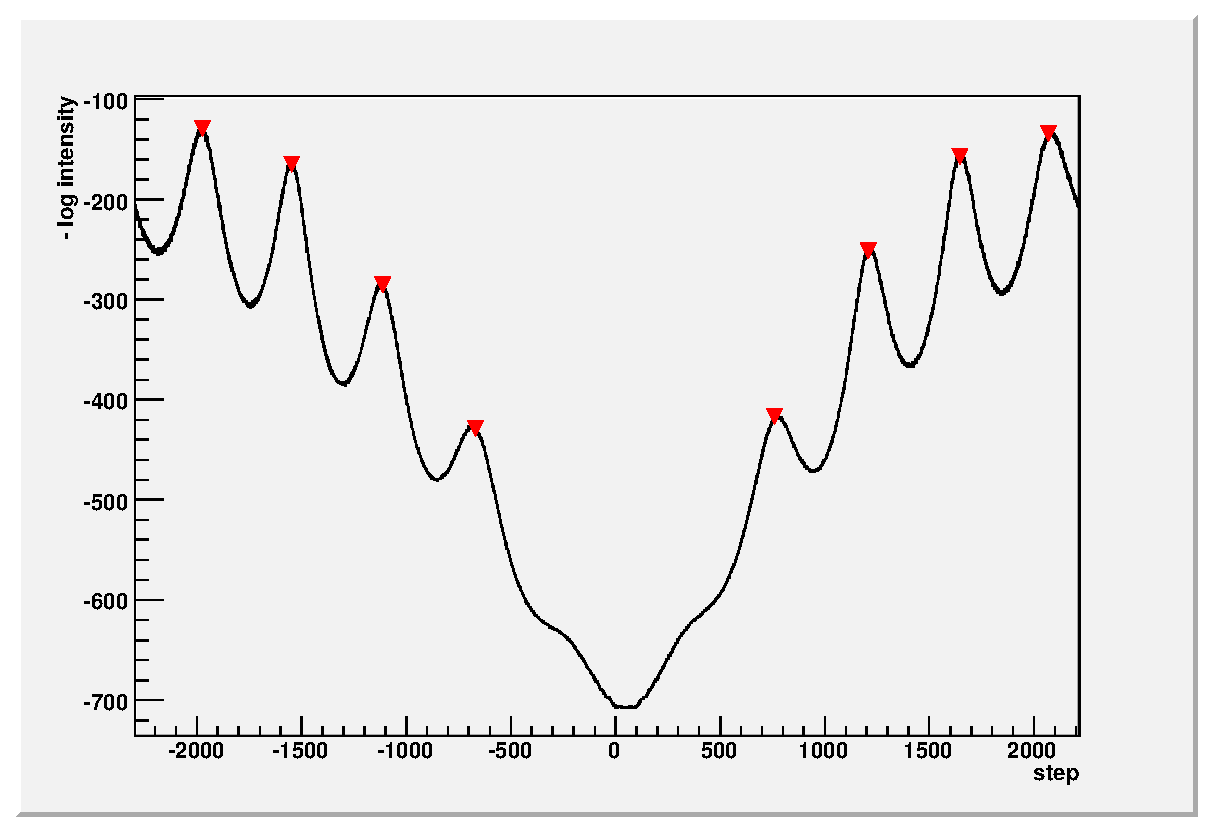
\includegraphics[scale=.6]{1slit.outint.eps}
\caption{Figura di diffrazione da una fenditura.}\label{1slitint}
\end{figure}
\begin{figure}[!h]\centering
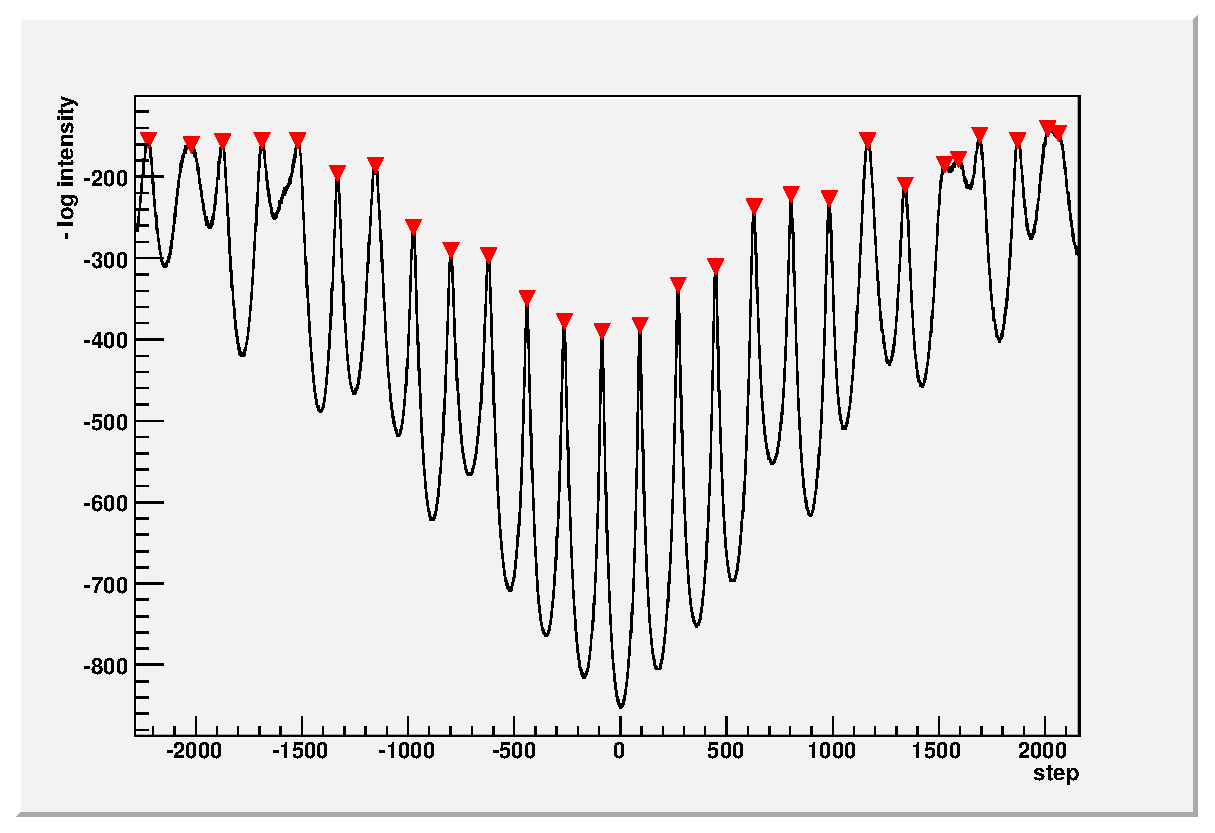
\includegraphics[scale=.6]{2slits.outint.eps}
\caption{Figura di interferenza da due fenditure.}\label{2slitsint}
\end{figure}
\begin{figure}[!h]\centering
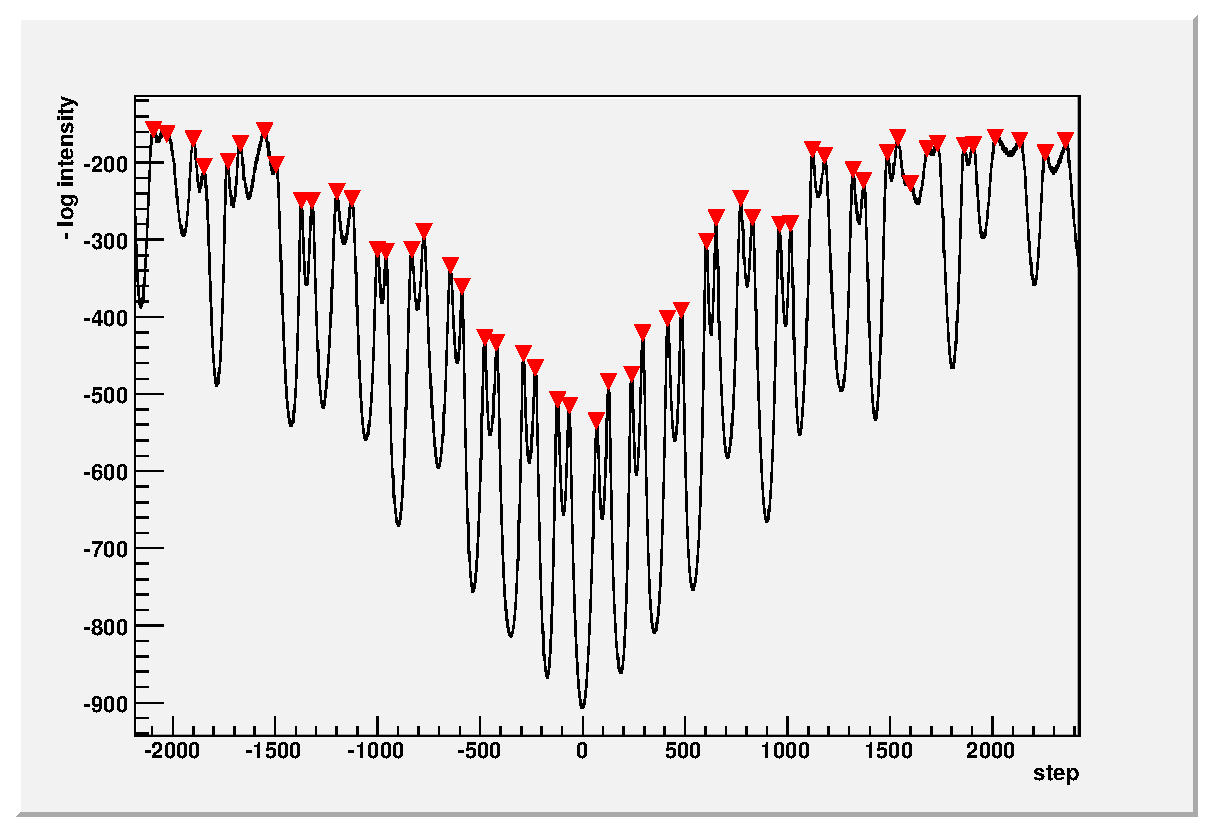
\includegraphics[scale=.6]{3slits.outint.eps}
\caption{Figura di interferenza da tre fenditure.}\label{3slitsint}
\end{figure}
\begin{figure}[!h]\centering
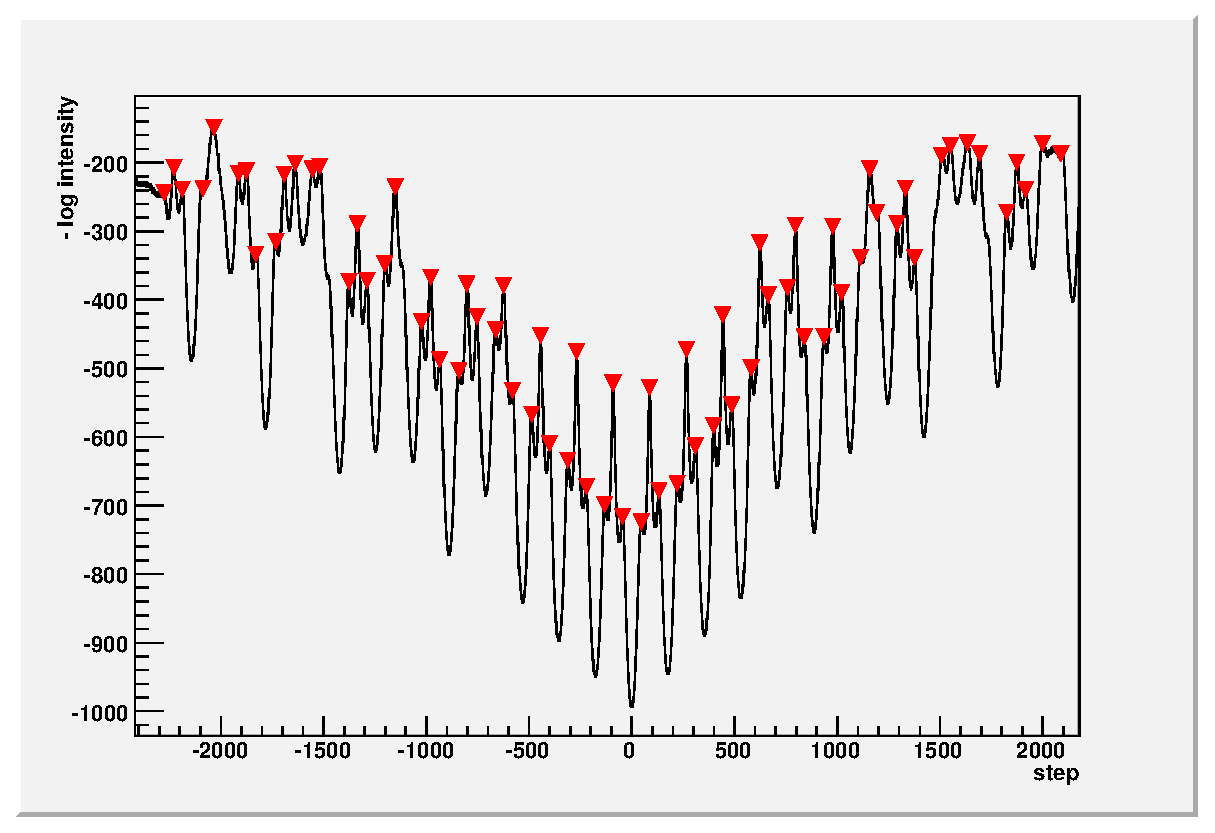
\includegraphics[scale=.6]{4slits.outint.eps}
\caption{Figura di interferenza da quattro fenditure.}\label{4slitsint}
\end{figure}

\begin{figure}[!h]\centering
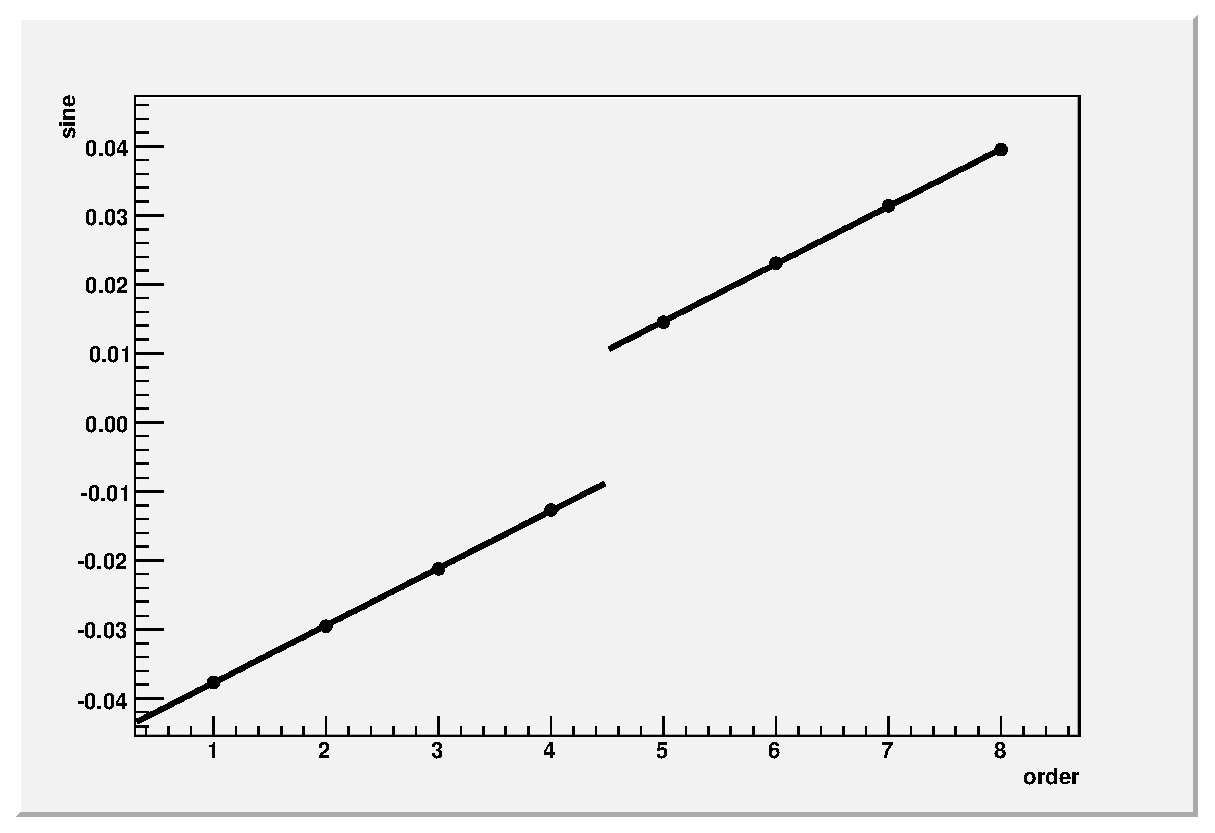
\includegraphics[scale=.6]{1slit.outsin.eps}
\caption{Diffrazione da una fenditura: grafico con numero d'ordine dei minimi in ascissa e seno dell'angolo di deflessione $\theta$ in ordinata. I due rami corrispondono ai minimi alla sinistra e alla destra del massimo centrale. Come si vede sono stati interpolati con due rette distinte.}\label{1slitsin}
\end{figure}
\begin{figure}[!h]\centering
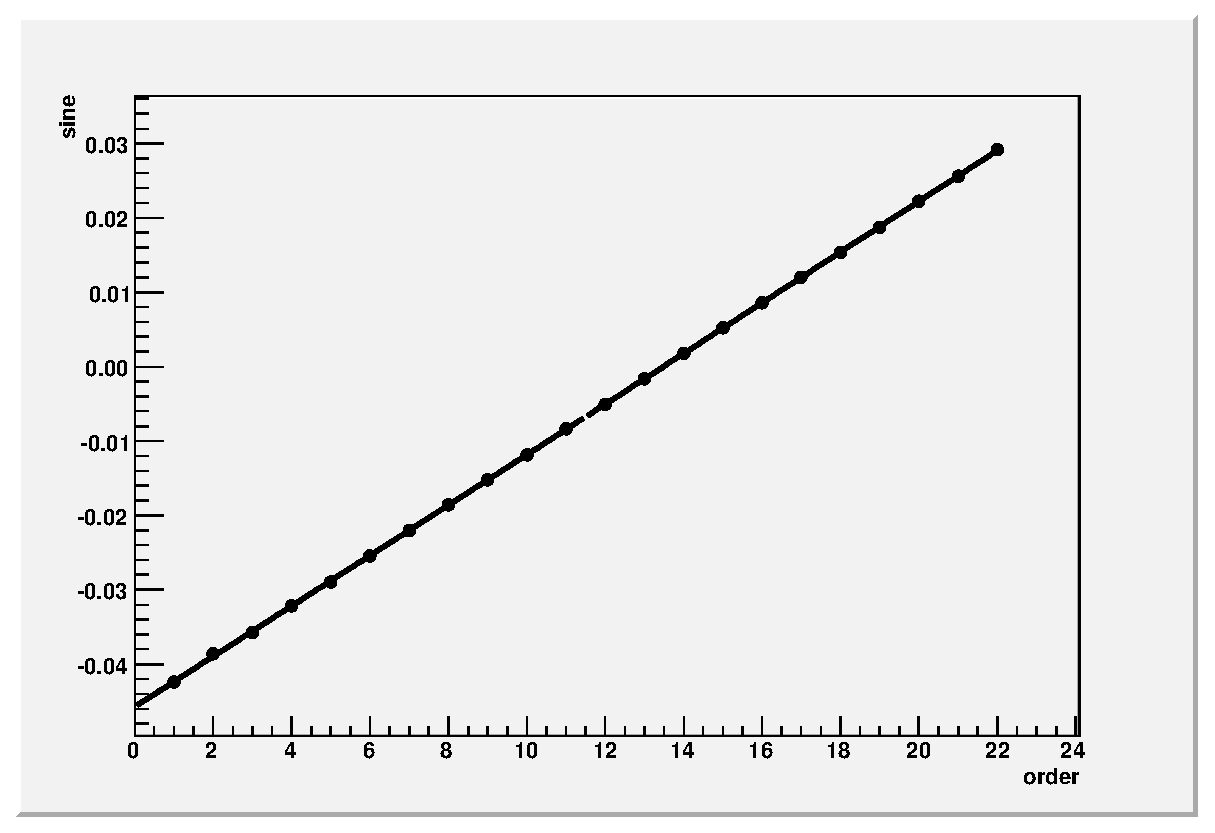
\includegraphics[scale=.6]{2slits.outsin.eps}
\caption{Interferenza da due fenditure: grafico con numero d'ordine dei minimi in ascissa e seno dell'angolo di deflessione $\theta$ in ordinata. I due rami corrispondono ai minimi alla sinistra e alla destra del massimo centrale, che sono stati interpolati con due rette distinte.}\label{2slitssin}
\end{figure}
\begin{figure}[!h]\centering
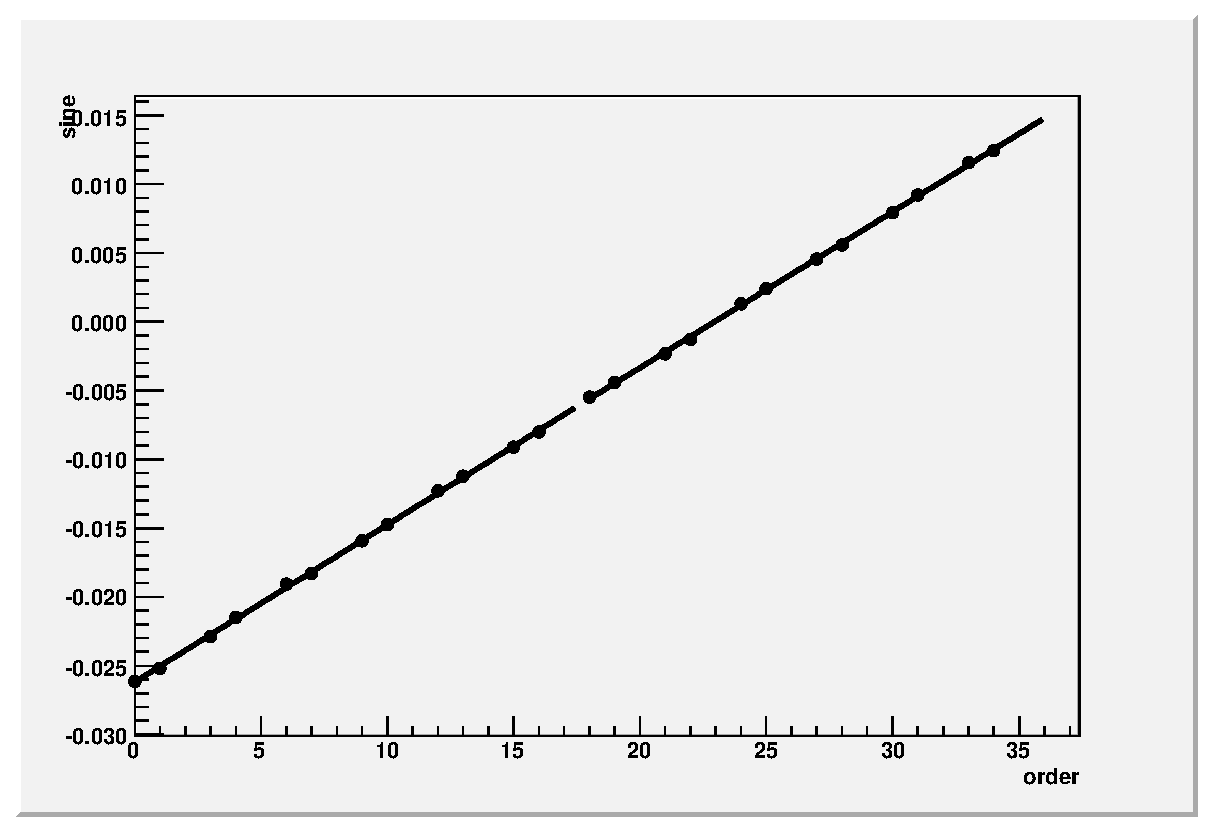
\includegraphics[scale=.6]{3slits.outsin.eps}
\caption{Interferenza da tre fenditure: grafico con numero d'ordine dei minimi in ascissa e seno dell'angolo di deflessione $\theta$ in ordinata. I due rami corrispondono ai minimi alla sinistra e alla destra del massimo centrale, che sono stati interpolati con due rette distinte.}\label{3slitssin}
\end{figure}
\begin{figure}[!h]\centering
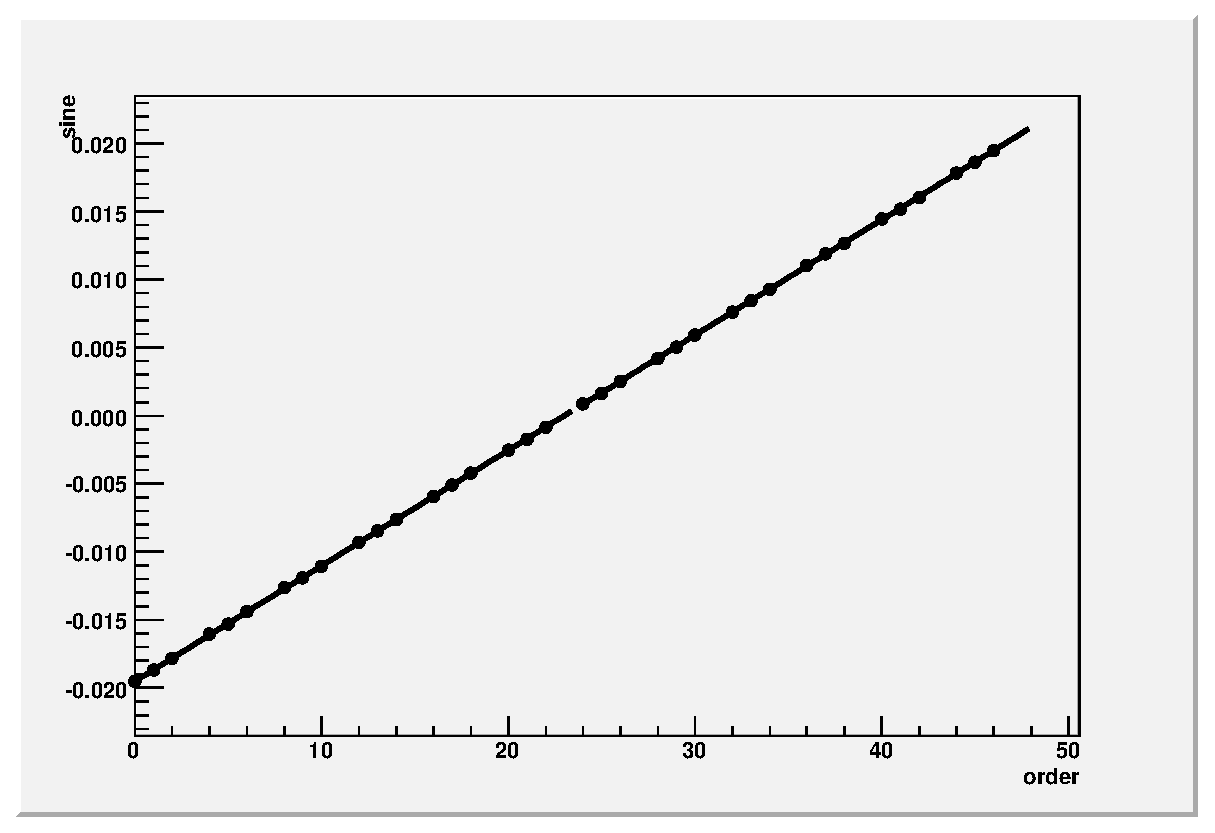
\includegraphics[scale=.6]{4slits.outsin.eps}
\caption{Interferenza da quattro fenditure: grafico con numero d'ordine dei minimi in ascissa e seno dell'angolo di deflessione $\theta$ in ordinata. I due rami corrispondono ai minimi alla sinistra e alla destra del massimo centrale, che sono stati interpolati con due rette distinte.}\label{4slitssin}
\end{figure}
\begin{figure}[!h]\centering
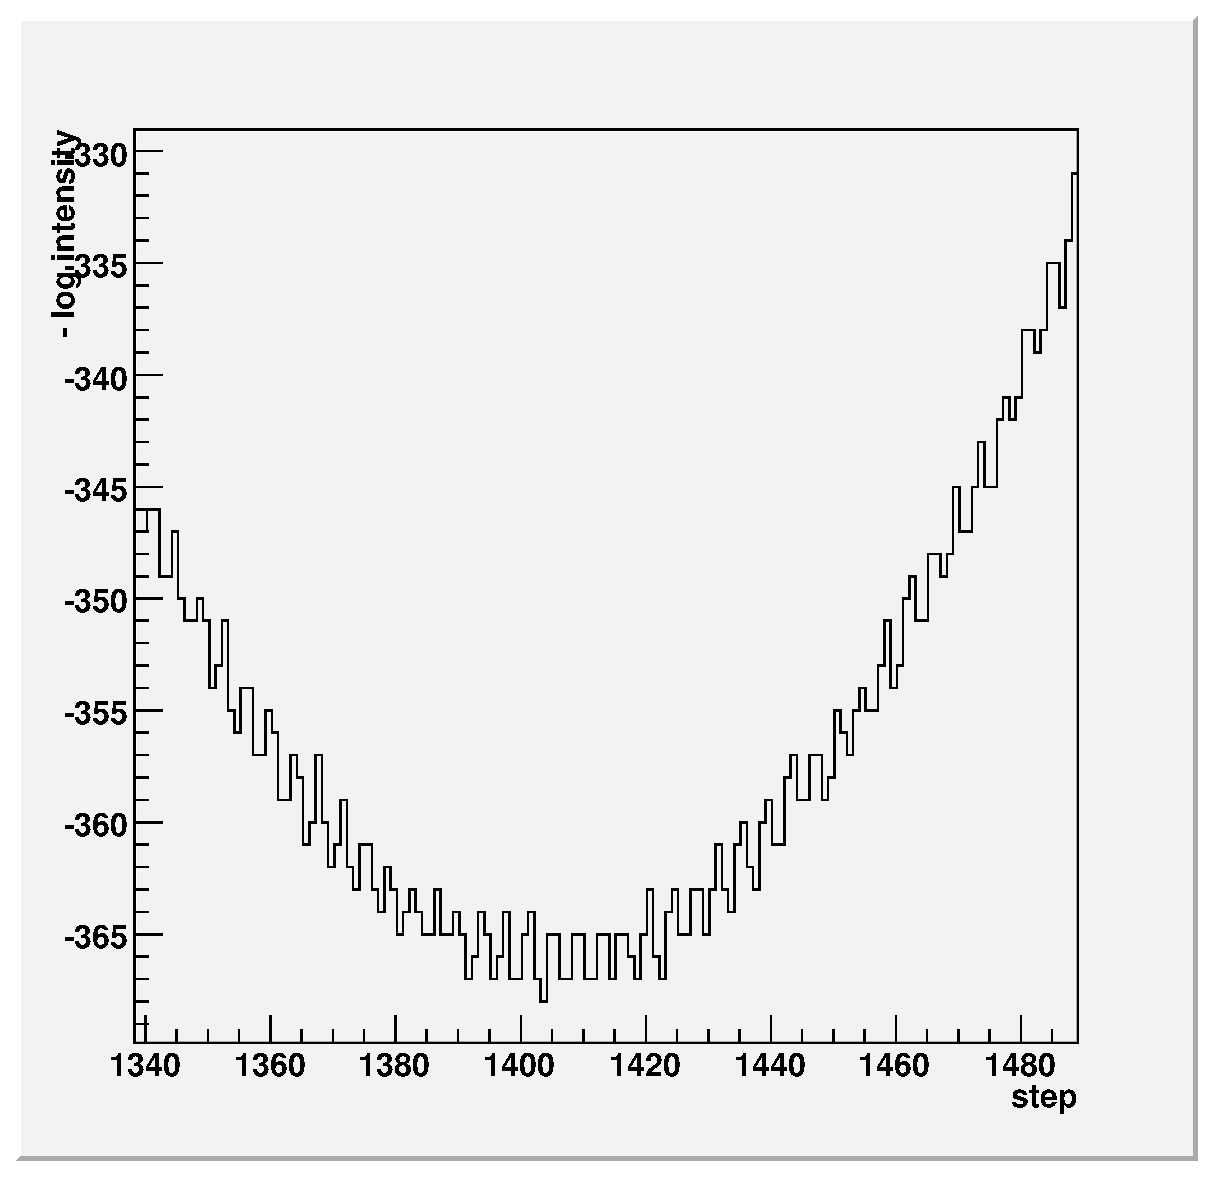
\includegraphics[scale=.6]{dentini.eps}
\caption{Ingrandimento di una porzione del grafico di diffrazione da singola fenditura. \`{E} evidente la fluttuazione casuale delle misure.}\label{dentini}
\end{figure}
\begin{figure}[!h]\centering
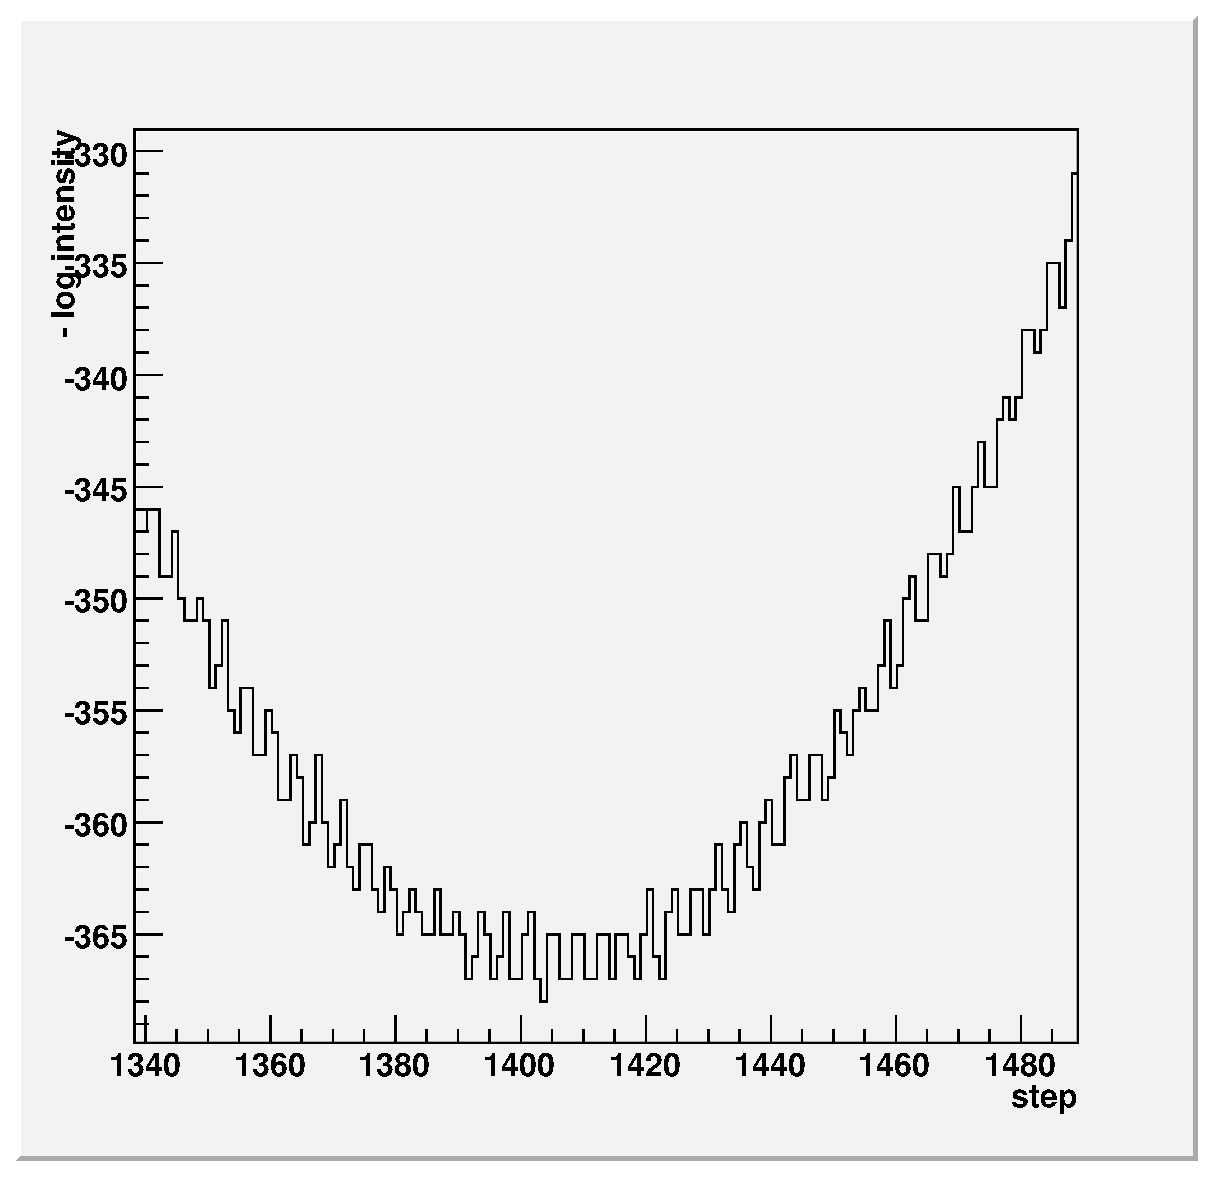
\includegraphics[scale=.6]{dentini.eps}
\caption{Ingrandimento di una porzione del grafico di diffrazione da singola fenditura. \`{E} evidente la fluttuazione casuale delle misure.}\label{dentini}
\end{figure}
\begin{figure}[!h]\centering
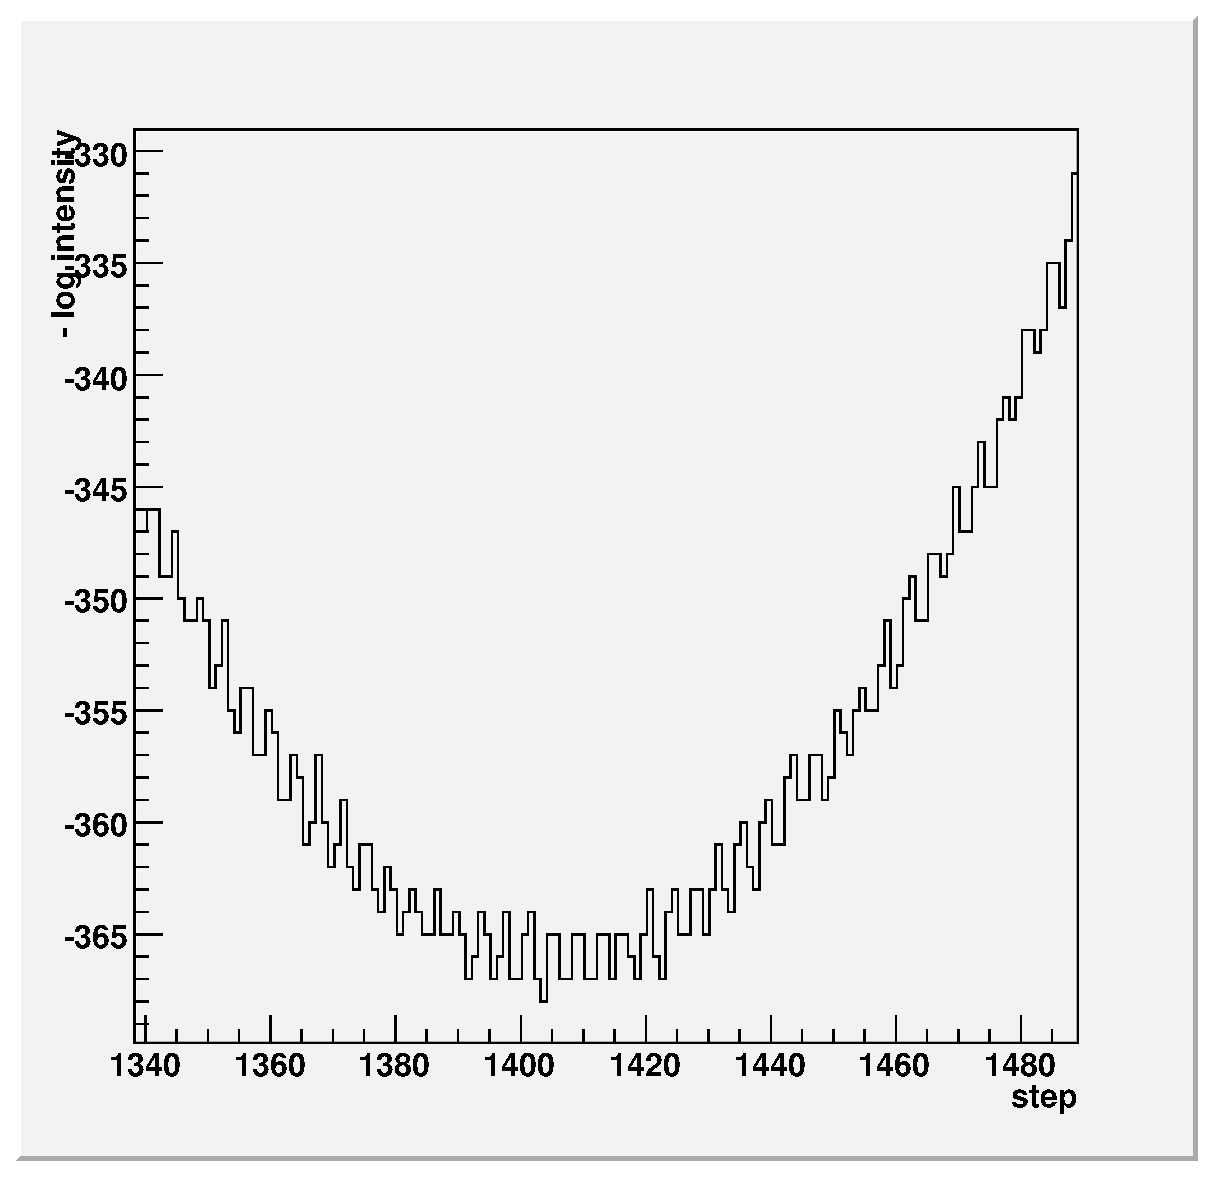
\includegraphics[scale=.6]{dentini.eps}
\caption{Ingrandimento di una porzione del grafico di diffrazione da singola fenditura. \`{E} evidente la fluttuazione casuale delle misure.}\label{dentini}
\end{figure}
\end{document}

